\documentclass{article}
\usepackage{tikz}
\usetikzlibrary{positioning}
\usetikzlibrary{decorations.markings}
\usepackage[dvipsnames]{xcolor}
\usepackage{amsmath}
\usepackage{pgfplots}

\begin{document}

\title{Matrizen in Neuronalen Netzwerken}
\author{Tim Zollner}
\date{17.02.2025}
\maketitle

\section{Feed-Forward}
\subsection{Grafik}
    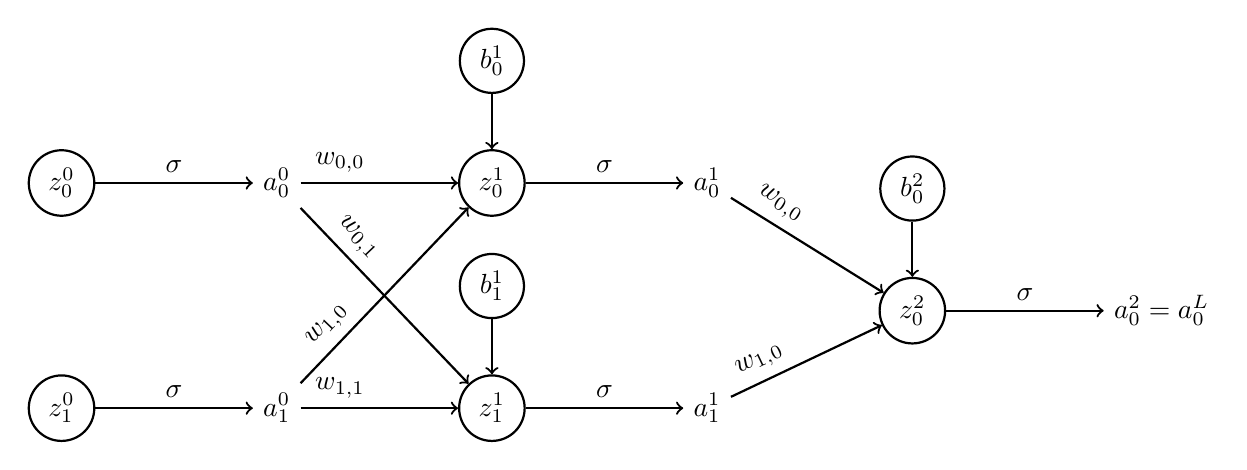
\begin{tikzpicture} [thick, main/.style = {draw, circle}]
        %Knoten
        \node[main] (z00) {$z_0^0$};
        \node[main] (z01) [below = 2cm of z00] {$z_1^0$};

        \node (a00) [right = 2cm of z00] {$a_0^0$};
        \node (a01) [right = 2cm of z01] {$a_1^0$};

        \node[main] (z10) [right = 2cm of a00] {$z_0^1$};
        \node[main] (z11) [right = 2cm of a01] {$z_1^1$};

        \node[main] (b10) [above = 0.7cm of z10] {$b_0^1$};
        \node[main] (b11) [above = 0.7cm of z11] {$b_1^1$};

        \node (a10) [right = 2cm of z10] {$a_0^1$};
        \node (a11) [right = 2cm of z11] {$a_1^1$};

        \node[main] (z20) [below right = 1cm and 2cm of a10] {$z_0^2$};
        \node[main] (b20) [above = 0.7cm of z20] {$b_0^2$};

        \node (a20) [right = 2cm of z20] {$a_0^2 = a_0^L$};

        %Kanten
        \draw[->] (z00) -- (a00) node[midway, above] {$\sigma$};
        \draw[->] (z01) -- (a01) node[midway, above] {$\sigma$};

        \draw[->] (a00) -- (z10) node[pos=0.25, above] {$w_{0,0}$};
        \draw[->] (a00) -- (z11) node[pos=0.25, above, sloped] {$w_{0,1}$};
        \draw[->] (a01) -- (z10) node[pos=0.25, above, sloped] {$w_{1,0}$};
        \draw[->] (a01) -- (z11) node[pos=0.25, above] {$w_{1,1}$};

        \draw[->] (b10) -- (z10);
        \draw[->] (b11) -- (z11);

        \draw[->] (z10) -- (a10) node[midway, above] {$\sigma$};
        \draw[->] (z11) -- (a11) node[midway, above] {$\sigma$};


        \draw[->] (a10) -- (z20) node[pos=0.25, above, sloped] {$w_{0,0}$};
        \draw[->] (a11) -- (z20) node[pos=0.25, above, sloped] {$w_{1,0}$};

        \draw[->] (b20) --(z20);

        \draw[->] (z20) -- (a20) node[midway, above] {$\sigma$};



    \end{tikzpicture}


\subsection{Formeln}
\[ z_0^1 = a_0^0 \cdot \textcolor{OliveGreen}{w_{0,0}} + a_1^0 \cdot \textcolor{OliveGreen}{w_{1,0}} + \textcolor{blue}{b^1} \]
allgemein:
\[  z_0^1 = \textcolor{blue}{b^1} + \sum_{j=0}^{n^1} a_j^0 \cdot \textcolor{OliveGreen}{w_{j,0}}  \]
\[a_j^l = \sigma(z_j^l)\]
\[\sigma(x) = \frac{1}{1 + e^{-x}}\]


\pagebreak
\subsection{Matrizendarstellung}
\[ \vec{z}^l = \left(\begin{array}{c} z_0^l \\ z_1^l \\ ... \\ z_j^l \end{array}\right) 
\kern 30pt
\vec{a}^l = \left(\begin{array}{c} a_0^l \\ a_1^l \\ ... \\ a_j^l \end{array}\right) 
\kern 30pt
\vec{b}^l = \left(\begin{array}{c} b_0^l \\ b_1^l \\ ... \\ b_j^l \end{array}\right) 
\kern 30pt
W^l = \begin{pmatrix}
    w_{0,0}^l & w_{1,0}^l & ... & w_{j,0}^l \\
    w_{0,1}^l & w_{1,1}^l & ... & w_{j,1}^l \\
    ... & ... & ... & ... \\
    w_{0,i}^l & w_{1,i}^l & ... & w_{j,i}^l
\end{pmatrix} \]

\[ \vec{a}^l = \vec{z}^{l-1} \cdot W^l + \vec{b}^l \]

\[ 
\left(\begin{array}{c} a_0^l \\ a_1^l \\ ... \\ a_j^l \end{array}\right)
=
\left(\begin{array}{c} z_0^{l-1} \\ z_1^{l-1} \\ ... \\ z_j^{l-1} \end{array}\right)
\cdot
\begin{pmatrix}
    w_{0,0}^l & w_{1,0}^l & ... & w_{j,0}^l \\
    w_{0,1}^l & w_{1,1}^l & ... & w_{j,1}^l \\
    ... & ... & ... & ... \\
    w_{0,i}^l & w_{1,i}^l & ... & w_{j,i}^l
\end{pmatrix}
+
\left(\begin{array}{c} b_0^l \\ b_1^l \\ ... \\ b_j^l \end{array}\right)
 \]

 \[
\left(\begin{array}{c} a_0^l \\ a_1^l \\ ... \\ a_j^l \end{array}\right)
=
\left(\begin{array}{c}
    w_{0,0}^l \cdot z_0^{l-1} + w_{1,0}^l \cdot z_1^{l-1} + ... + w_{j,0}^l \cdot z_j^{l-1} \\
    w_{0,1}^l \cdot z_0^{l-1} + w_{1,1}^l \cdot z_1^{l-1} + ... + w_{j,1}^l \cdot z_j^{l-1} \\
    ... \\
    w_{0,i}^l \cdot z_0^{l-1} + w_{1,i}^l \cdot z_1^{l-1} + ... + w_{j,i}^l \cdot z_j^{l-1}
\end{array}\right)
+
\left(\begin{array}{c} b_0^l \\ b_1^l \\ ... \\ b_j^l \end{array}\right)\]


\newpage
\section{Backpropagation}
\subsection{Verlustfunktion}
\[ E_j = \frac{1}{2}(y_j - a_j^L)^2 \]
\[ E = \frac{1}{2}\sum_{j}^{} (y_j - a_j^L)^2 \]
\[ \frac{dE_j}{da_{j}^L}  = (a_j^L - y_j) \]


\subsection{Lernvorgang}
Anpassen der Gewichts- und BiasNeuronen:

\[ w^l = w^l - \frac{\eta}{N} \cdot \sum_{k = 0}^{N} \frac{\partial C^k}{\partial w^l} \]
$\eta$ = Lernrate \kern 20pt $N$ = Anzahl der Trainingsbeispiele \kern 20pt $k$ = Trainingsbeispiel 


\subsection{Ableitung der sigmoid Funktion}
\[ \textcolor{blue}{ \sigma(x) = \frac{1}{1 + e^{-x}} } \]
\[ \textcolor{red}{ \frac{d}{dx}\sigma(x) } = \frac{
0( \cdot 1 + e^{-x}) - 1 \cdot e^{-x} \cdot -1
}{
    (1 + e^{-x})^2
} = \frac{e^{-x}}{(1 + e^{-x})^2} 
= \frac{1 + e^{-x} - 1}{(1 + e^{-x})^2} \]
\[ =\frac{1 + e^{-x}}{(1 + e^{-x})^2} - \frac{1}{(1 + e^{-x})^2} 
= \frac{1}{1 + e^{-x}} - \frac{1}{(1 + e^{-x})^2} \]
\[ = \frac{1}{1 + e^{-x}} \cdot (1 - \frac{1}{1 + e^{-x}}) 
= \textcolor{red}{ \sigma(x) \cdot (1 - \sigma(x)) } \]

\resizebox{280pt}{210pt}{
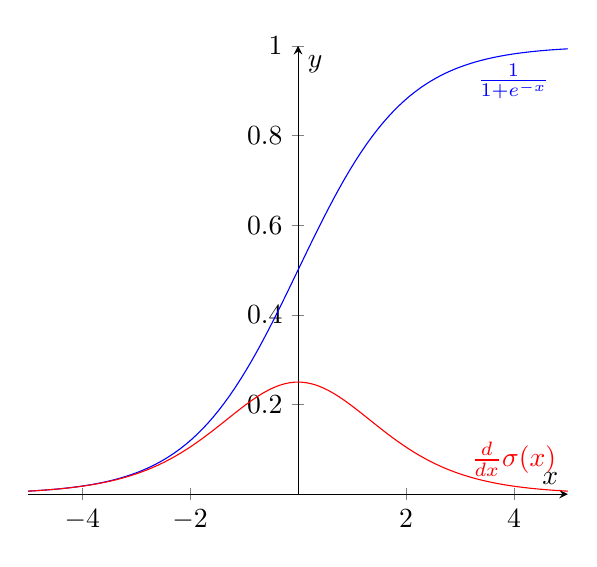
\begin{tikzpicture}[>=stealth]
    \begin{axis}[
        xmin=-5,xmax=5,
        ymin=0,ymax=1,
        axis x line=middle,
        axis y line=middle,
        axis line style=->,
        xlabel={$x$},
        ylabel={$y$},
    ]
    \addplot[no marks, blue] expression[domain=-5:5, samples=100]{1 / (1+ exp(-x))}
    node[pos=0.9, below] {$\frac{1}{1 + e^{-x}}$};
    \addplot[no marks, red] expression[domain=-5:5, samples=100]{1 / (1+ exp(-x)) * (1 - 1 / (1+ exp(-x)))}
    node[pos=0.9, above] {$\frac{d}{dx} \sigma(x)$};

    \end{axis}
\end{tikzpicture}
}


\subsection{Fehler($\delta$)}
-Zwischenwert zur leichteren Berechnung des Gradienten
\[ \delta_j^l = \frac{\partial E}{\partial z_j^l} 
\kern 40pt
 \frac{\partial E}{\partial w_{j,i}^l} = \delta_i^l \cdot a_j^{l-1}
\kern 40pt
\frac{\partial E}{\partial b_j^l} = \delta_j^l \]

Berechnung des Fehlers des letzten Layers durch Anwendung der Kettenregel:
\[ \delta_j^L  = \frac{\partial E}{\partial z_j^L}
= \frac{\partial E}{\partial a_j^L} \cdot \frac{\partial a_j^L}{\partial z_j^L}\]
Einsetzen der Ableitungen:
\[ = \frac{\partial E}{\partial a_j^L} \cdot \sigma (z_j^L) \cdot (1 - \sigma (z_j^L)) \]
\[ = (a_j^L - y_j) \cdot \sigma (z_j^L) \cdot (1 - \sigma (z_j^L)) \]

Berechnung des Fehlers des vorletzten Layers:

\[ \delta_j^{L-1}  = \frac{\partial E}{\partial z_j^{L-1}} 
= \textcolor{OliveGreen}{\frac{\partial E}{\partial a_j^{L-1}}} \cdot \textcolor{blue}{\frac{\partial a_j^{L-1}}{\partial z_j^{L-1}}} \]

\[ \textcolor{blue}{\frac{\partial a_j^{L-1}}{\partial z_j^{L-1}} = \sigma^{\prime}(z_j^{L-1})} \]

\[ \textcolor{OliveGreen}{ \frac{\partial E}{\partial a_j^{L-1}} = \sum_{i 
= 0}^{n^L} \frac{\partial E}{\partial z_i^L} \cdot \frac{\partial z_i^L}{\partial a_j^{L-1}} }
= \sum_{i = 0}^{n^L} \delta_i^L \cdot \textcolor{red}{ \frac{\partial z_i^L}{\partial a_j^{L-1}} } \]

\[ \textcolor{red}{ \frac{\partial z_i^L}{\partial a_j^{L-1}}
= \frac{\partial}{\partial a_j^{L-1}} (\sum_{p = 0}^{n^L} a_p^{L-1} \cdot w_{p,i}^L + b_p^L) = w_{j, i}^L } \]

\[ \textcolor{OliveGreen}{ \frac{\partial E}{\partial a_j^{L-1}} } = \sum_{i = 0}^{n^L} \delta_j^L \cdot \textcolor{red}{ w_{j,i}^L } \]

Zusammenführen der Einzelergebnisse:
\[ \delta_j^{L-1} = \textcolor{OliveGreen}{[\sum_{i = 0}^{n^{L}} \delta_j^{L} \cdot w_{j,i}^{L} } \cdot \textcolor{blue}{ \sigma^{\prime}(z_j^{L-1}) } \]
Allgemein:
\[ \delta_j^{l} = \textcolor{OliveGreen}{ [\sum_{i = 0}^{n^{l+1}} \delta_j^{l+1} \cdot w_{j,i}^{l+1}] } \cdot \textcolor{blue}{ \sigma^{\prime}(z_j^{l}) } \]


\subsection{Berechnung des Fehlers als Vektor}


\subsubsection{Fehler des letzten Layers}
\[ \delta_j^L = (a_j^L - y_j) \cdot \sigma^{\prime} (z_j^L)  \]

\[ \vec{\delta^L} = \left( \begin{array}{c}
     \delta_0^L \\ \delta_1^L \\ ... \\ \delta_j^L 
\end{array} \right)
\kern 30pt
\vec{y} = \left( \begin{array} {c}
    y_0 \\ y_1 \\ ... \\ y_j
\end{array} \right) 
\kern 30pt
\vec{a^L} = \left(\begin{array}{c}
    a_0^L \\ a_1^L \\ ... \\ a_j^L
\end{array} \right) 
\kern 30pt
\vec{z^L} = \left(\begin{array}{c}
    z_0^L \\ z_1^L \\ ... \\ z_j^L
\end{array} \right) 
\]

\[ \vec{\delta^L} = (\vec{a^L} - \vec{y^L}) \odot \sigma^{\prime}(\vec{z^L}) \]


\subsubsection{Definition $\odot$}
\[ \left(\begin{array}{c}
    a_0 \\ a_1 \\ a_2 \\ a_3
\end{array}\right)
\odot \left(\begin{array}{c}
    b_0 \\ b_1 \\ b_2 \\ b_3
\end{array}\right) 
= \left(\begin{array}{c}
    a_0 \cdot b_0 \\ a_1 \cdot b_1 \\ a_2 \cdot b_2 \\ a_3 \cdot b_3
\end{array}\right) \]


\subsubsection{Fehler eines beliebigen Layers}
\[ \delta_j^{l} = [\sum_{i = 0}^{n^{l+1}} \delta_j^{l+1} \cdot w_{j,i}^{l+1}] \cdot \sigma^{\prime}(z_j^{l})  \]


\end{document}